\documentclass{standalone}
\usepackage{tikz}
\usetikzlibrary{patterns, positioning}


\begin{document}
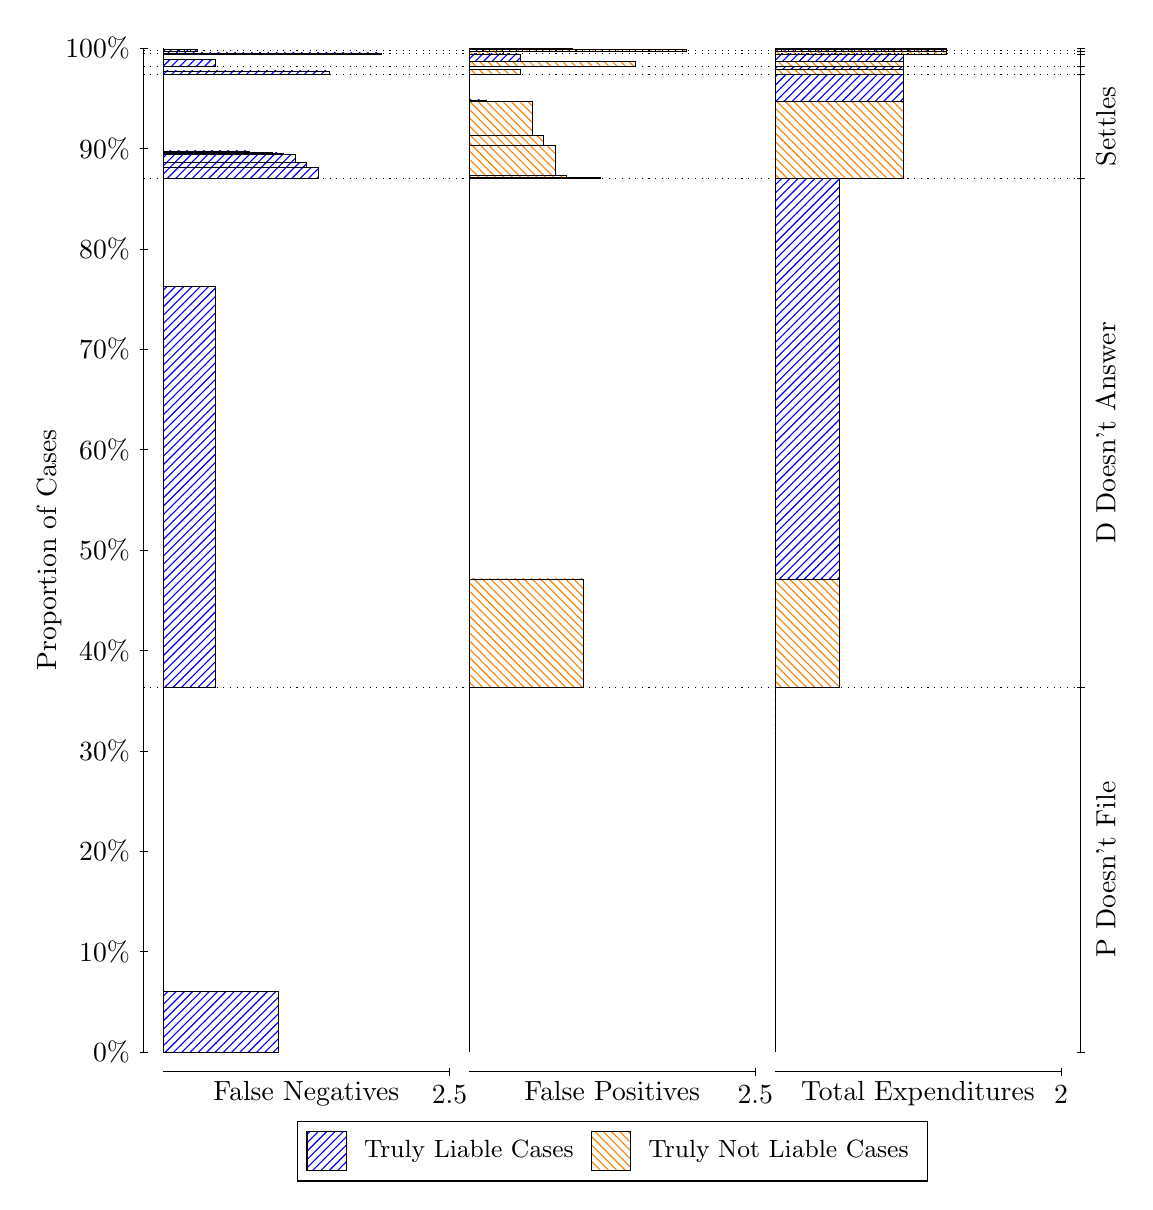
\begin{tikzpicture}
\draw[black, very thin] (1.5,1.75) -- (1.5,14.5);
\node[rotate=90, text=black, anchor=center] at (0.3, 8.125) {Proportion of Cases};
\draw[black, very thin] (1.45,1.75) -- (1.55,1.75);
\node[text=black, anchor=east] at (1.45, 1.75) {0\%};
\draw[black, very thin] (1.45,3.025) -- (1.55,3.025);
\node[text=black, anchor=east] at (1.45, 3.025) {10\%};
\draw[black, very thin] (1.45,4.3) -- (1.55,4.3);
\node[text=black, anchor=east] at (1.45, 4.3) {20\%};
\draw[black, very thin] (1.45,5.575) -- (1.55,5.575);
\node[text=black, anchor=east] at (1.45, 5.575) {30\%};
\draw[black, very thin] (1.45,6.85) -- (1.55,6.85);
\node[text=black, anchor=east] at (1.45, 6.85) {40\%};
\draw[black, very thin] (1.45,8.125) -- (1.55,8.125);
\node[text=black, anchor=east] at (1.45, 8.125) {50\%};
\draw[black, very thin] (1.45,9.4) -- (1.55,9.4);
\node[text=black, anchor=east] at (1.45, 9.4) {60\%};
\draw[black, very thin] (1.45,10.675) -- (1.55,10.675);
\node[text=black, anchor=east] at (1.45, 10.675) {70\%};
\draw[black, very thin] (1.45,11.95) -- (1.55,11.95);
\node[text=black, anchor=east] at (1.45, 11.95) {80\%};
\draw[black, very thin] (1.45,13.225) -- (1.55,13.225);
\node[text=black, anchor=east] at (1.45, 13.225) {90\%};
\draw[black, very thin] (1.45,14.5) -- (1.55,14.5);
\node[text=black, anchor=east] at (1.45, 14.5) {100\%};

\draw[black, very thin] (13.4,1.75) -- (13.4,14.5);
\draw[black, very thin] (13.35,1.75) -- (13.45,1.75);
\node[anchor=west] at (13.35, 1.75) {};
\draw[black, very thin] (13.35,6.3826) -- (13.45,6.3826);
\node[anchor=west] at (13.35, 6.3826) {};
\draw[black, very thin] (13.35,12.844) -- (13.45,12.844);
\node[anchor=west] at (13.35, 12.844) {};
\draw[black, very thin] (13.35,14.169) -- (13.45,14.169);
\node[anchor=west] at (13.35, 14.169) {};
\draw[black, very thin] (13.35,14.266) -- (13.45,14.266);
\node[anchor=west] at (13.35, 14.266) {};
\draw[black, very thin] (13.35,14.425) -- (13.45,14.425);
\node[anchor=west] at (13.35, 14.425) {};
\draw[black, very thin] (13.35,14.465) -- (13.45,14.465);
\node[anchor=west] at (13.35, 14.465) {};
\draw[black, very thin] (13.35,14.5) -- (13.45,14.5);
\node[anchor=west] at (13.35, 14.5) {};

\draw[black, very thin, pattern color=blue, pattern=north east lines] (1.75,1.75) rectangle (3.2033,2.5221);
\draw[black, very thin, pattern color=orange, pattern=north west lines] (1.75,2.5221) rectangle (1.75,6.3826);
\draw[black, very thin, pattern color=blue, pattern=north east lines] (1.75,6.3826) rectangle (2.404,11.469);
\draw[black, very thin, pattern color=orange, pattern=north west lines] (1.75,11.469) rectangle (1.75,12.844);
\draw[black, very thin, pattern color=blue, pattern=north east lines] (1.75,12.844) rectangle (3.712,12.988);
\draw[black, very thin, pattern color=blue, pattern=north east lines] (1.75,12.988) rectangle (3.5667,13.047);
\draw[black, very thin, pattern color=blue, pattern=north east lines] (1.75,13.047) rectangle (3.4213,13.145);
\draw[black, very thin, pattern color=blue, pattern=north east lines] (1.75,13.145) rectangle (3.276,13.169);
\draw[black, very thin, pattern color=blue, pattern=north east lines] (1.75,13.169) rectangle (3.1307,13.17);
\draw[black, very thin, pattern color=blue, pattern=north east lines] (1.75,13.17) rectangle (2.84,13.194);
\draw[black, very thin, pattern color=orange, pattern=north west lines] (1.75,13.194) rectangle (1.75,14.169);
\draw[black, very thin, pattern color=blue, pattern=north east lines] (1.75,14.169) rectangle (3.8573,14.209);
\draw[black, very thin, pattern color=orange, pattern=north west lines] (1.75,14.209) rectangle (1.75,14.266);
\draw[black, very thin, pattern color=blue, pattern=north east lines] (1.75,14.266) rectangle (2.404,14.357);
\draw[black, very thin, pattern color=orange, pattern=north west lines] (1.75,14.357) rectangle (1.75,14.425);
\draw[black, very thin, pattern color=blue, pattern=north east lines] (1.75,14.425) rectangle (4.5113,14.438);
\draw[black, very thin, pattern color=orange, pattern=north west lines] (1.75,14.438) rectangle (1.75,14.465);
\draw[black, very thin, pattern color=blue, pattern=north east lines] (1.75,14.465) rectangle (2.186,14.487);
\draw[black, very thin, pattern color=orange, pattern=north west lines] (1.75,14.487) rectangle (1.75,14.5);
\draw[black, very thin, pattern color=orange, pattern=north west lines] (5.6333,1.75) rectangle (5.6333,5.6105);
\draw[black, very thin, pattern color=blue, pattern=north east lines] (5.6333,5.6105) rectangle (5.6333,6.3826);
\draw[black, very thin, pattern color=orange, pattern=north west lines] (5.6333,6.3826) rectangle (7.0867,7.7572);
\draw[black, very thin, pattern color=blue, pattern=north east lines] (5.6333,7.7572) rectangle (5.6333,12.844);
\draw[black, very thin, pattern color=orange, pattern=north west lines] (5.6333,12.844) rectangle (7.3047,12.853);
\draw[black, very thin, pattern color=orange, pattern=north west lines] (5.6333,12.853) rectangle (7.014,12.853);
\draw[black, very thin, pattern color=orange, pattern=north west lines] (5.6333,12.853) rectangle (6.8687,12.878);
\draw[black, very thin, pattern color=orange, pattern=north west lines] (5.6333,12.878) rectangle (6.7233,13.263);
\draw[black, very thin, pattern color=orange, pattern=north west lines] (5.6333,13.263) rectangle (6.578,13.391);
\draw[black, very thin, pattern color=orange, pattern=north west lines] (5.6333,13.391) rectangle (6.4327,13.818);
\draw[black, very thin, pattern color=blue, pattern=north east lines] (5.6333,13.818) rectangle (5.8513,13.842);
\draw[black, very thin, pattern color=blue, pattern=north east lines] (5.6333,13.842) rectangle (5.6333,14.169);
\draw[black, very thin, pattern color=orange, pattern=north west lines] (5.6333,14.169) rectangle (6.2873,14.226);
\draw[black, very thin, pattern color=blue, pattern=north east lines] (5.6333,14.226) rectangle (5.6333,14.266);
\draw[black, very thin, pattern color=orange, pattern=north west lines] (5.6333,14.266) rectangle (7.7407,14.335);
\draw[black, very thin, pattern color=blue, pattern=north east lines] (5.6333,14.335) rectangle (6.2873,14.425);
\draw[black, very thin, pattern color=orange, pattern=north west lines] (5.6333,14.425) rectangle (6.0693,14.453);
\draw[black, very thin, pattern color=blue, pattern=north east lines] (5.6333,14.453) rectangle (5.6333,14.465);
\draw[black, very thin, pattern color=orange, pattern=north west lines] (5.6333,14.465) rectangle (8.3947,14.478);
\draw[black, very thin, pattern color=blue, pattern=north east lines] (5.6333,14.478) rectangle (6.9413,14.5);
\draw[black, very thin, pattern color=orange, pattern=north west lines] (9.5167,1.75) rectangle (9.5167,5.6105);
\draw[black, very thin, pattern color=blue, pattern=north east lines] (9.5167,5.6105) rectangle (9.5167,6.3826);
\draw[black, very thin, pattern color=orange, pattern=north west lines] (9.5167,6.3826) rectangle (10.334,7.7572);
\draw[black, very thin, pattern color=blue, pattern=north east lines] (9.5167,7.7572) rectangle (10.334,12.844);
\draw[black, very thin, pattern color=orange, pattern=north west lines] (9.5167,12.844) rectangle (11.152,13.818);
\draw[black, very thin, pattern color=blue, pattern=north east lines] (9.5167,13.818) rectangle (11.152,14.169);
\draw[black, very thin, pattern color=orange, pattern=north west lines] (9.5167,14.169) rectangle (11.152,14.226);
\draw[black, very thin, pattern color=blue, pattern=north east lines] (9.5167,14.226) rectangle (11.152,14.266);
\draw[black, very thin, pattern color=orange, pattern=north west lines] (9.5167,14.266) rectangle (11.152,14.335);
\draw[black, very thin, pattern color=blue, pattern=north east lines] (9.5167,14.335) rectangle (11.152,14.425);
\draw[black, very thin, pattern color=orange, pattern=north west lines] (9.5167,14.425) rectangle (11.697,14.453);
\draw[black, very thin, pattern color=blue, pattern=north east lines] (9.5167,14.453) rectangle (11.697,14.465);
\draw[black, very thin, pattern color=orange, pattern=north west lines] (9.5167,14.465) rectangle (11.697,14.478);
\draw[black, very thin, pattern color=blue, pattern=north east lines] (9.5167,14.478) rectangle (11.697,14.5);
\draw[black, dotted] (1.5,6.3826) -- (13.4,6.3826);
\draw[black, dotted] (1.5,12.844) -- (13.4,12.844);
\draw[black, dotted] (1.5,14.169) -- (13.4,14.169);
\draw[black, dotted] (1.5,14.266) -- (13.4,14.266);
\draw[black, dotted] (1.5,14.425) -- (13.4,14.425);
\draw[black, dotted] (1.5,14.465) -- (13.4,14.465);
\draw[black, very thin] (1.75,1.5) -- (5.3833,1.5);
\node[text=black, anchor=north] at (3.5667, 1.5) {False Negatives};
\draw[black, very thin] (5.3833,1.45) -- (5.3833,1.55);
\node[text=black, anchor=north] at (5.3833, 1.45) {2.5};

\draw[black, very thin] (5.6333,1.5) -- (9.2667,1.5);
\node[text=black, anchor=north] at (7.45, 1.5) {False Positives};
\draw[black, very thin] (9.2667,1.45) -- (9.2667,1.55);
\node[text=black, anchor=north] at (9.2667, 1.45) {2.5};

\draw[black, very thin] (9.5167,1.5) -- (13.15,1.5);
\node[text=black, anchor=north] at (11.333, 1.5) {Total Expenditures};
\draw[black, very thin] (13.15,1.45) -- (13.15,1.55);
\node[text=black, anchor=north] at (13.15, 1.45) {2};

\node[text=black, centered, rotate=90] at (13.72, 4.0663) {P Doesn't File};
\node[text=black, centered, rotate=90] at (13.72, 9.6131) {D Doesn't Answer};
\node[text=black, centered, rotate=90] at (13.72, 13.506) {Settles};





\draw (7.449999999999999,1.5) node[draw=none] (baseCoordinate) {};
\begin{scope}[align=center]
        \matrix[scale=0.5, draw=black, below=0.5cm of baseCoordinate, nodes={draw}, column sep=0.1cm]{
            \node[rectangle, draw, minimum width=0.5cm, minimum height=0.5cm, pattern color=blue, pattern=north east lines] {}; &
            \node[draw=none, font=\small, text=black] (B) {Truly Liable Cases}; &
            \node[rectangle, draw, minimum width=0.5cm, minimum height=0.5cm, pattern color=orange, pattern=north west lines] {}; &
            \node[draw=none, font=\small, text=black] (B) {Truly Not Liable Cases}; \\
            };
\end{scope}

\end{tikzpicture}
\end{document}